
\chapter{Realizacja} \label{chap:realization}
W tym rozdziale zostały opisane realizacje elementów opisanych w koncepcji z rozdziału \ref{chap:methodology}. Ze względu na to, że realizacja części elementów została przeprowadzona z użyciem podobnych bądź tych samych narzędzi czy algorytmów, zostały one zagregowane i opisane w sekcji \ref{sec:tools}. W dalszych sekcjach zostały przedstawione kolejno:
\begin{itemize}
    \item proces zbierania i analizowania danych oraz próba uzupełnienia danych brakujących,
    \item budowa modeli predykcyjnych z wykorzystaniem różnych podejść i algorytmów,
    \item opis realizacji optymalizacji heurystycznej,
    \item prezentacja systemu wspomagania decyzji.
\end{itemize}

\section{Zbiór i opis narzędzi oraz algorytmów użytych podczas realizacji}\label{sec:tools}
\subsection{Analiza oraz modelowanie danych}\label{sec:tools-data-analysis-modeling}
Do tej części pracy zostały wykorzystane narzędzia, których miałem okazję użyć podczas projektów związanych z eksploracją danych oraz na zajęciach z uczenia maszynowego. Wybór został podyktowany niskim progiem wejścia lub ominięciem etapu poznawania nowych narzędzi.
\newpage
Lista użytych narzędzi:
\begin{itemize}
    \item Microsoft Office Excel\footnote{\url{https://www.microsoft.com/pl-pl/microsoft-365/excel}} - oprogramowanie użyte na potrzeby gromadzenia oraz edycji danych podczas budowy zbioru danych,
    \item Język programowania Python\footnote{\url{https://www.python.org/}} w wersji 3.7 - język interpretowany wysokiego poziomu, został wybrany ze względu na ogromną społeczność programistów oraz masę bibliotek wspomagających procesy analizy oraz modelowania danych,
    \item Jupyter Lab\footnote{\url{https://jupyter.org/}} - środowisko programistyczne dla języka Python uruchamiane w przeglądarce internetowej, umożliwia podzielenie kodu na komórki oraz wykonywanie ich wraz z prezentacją wyników,
    \item Pandas\footnote{\url{https://pandas.pydata.org/}} - narzędzie dla języka Python wspomagające analizę oraz manipulację danymi,
    \item Matplotlib\footnote{\url{https://matplotlib.org/}} - biblioteka dla języka Python umożliwiająca tworzenie wykresów,
    \item Scikit-learn\footnote{\url{https://scikit-learn.org/}} \cite{scikit-learn} - narzędzie dla języka Python dostarczające algorytmów służacych do budowy modeli uczenia maszynowego,
    \item TensorFlow\footnote{\url{https://www.tensorflow.org/}} \cite{tensorflow2015-whitepaper} - otwartoźródłowa platforma służąca do budowania modeli uczenia maszynowego, została wykorzystana do budowy sieci neuronowych ze względu na dobrze udokumentowany interfejs programistyczny Keras API\footnote{\url{https://keras.io/}} pozwalający na proste i szybkie definiowanie architektury modeli,
    \item XGBoost\footnote{\url{https://xgboost.ai/}} \cite{xgboost} -  biblioteka dostarczająca imlementację algorytmu gradient boostingu, która została zoptymalizowana pod kątem szybkości działania oraz jakości przewidywań, udostępnia API pozwalające używać jej z wykorzystaniem narzędzia scikit-learn.
\end{itemize}

Użyte algorytmy wraz ze skróconym opisem działania:
\begin{itemize}
    \item k-krotna walidacja krzyżowa \cite{crossvalidation} - metoda służąca do badania jakości wytrenowanych modeli poprzez podzielenie zbioru danych na k części i użycie jednego z podzbiorów jako zbioru testowego a pozostałych jako zbióe treningowy,
    \item Random Forest \cite{random_forest} - algorytm służący do budowania klasyfikatorów oraz regresorów  za pomocą ensemblingu drzew decyzyjnych, w którym każde z drzew jest budowane za pomocą próbkowania z podmianą ze zbioru treningowego,
    \item Gradient Boosting \cite{gradient_boosting} - algorytm służący do budowania klasyfikatorów oraz regresorów, w którym każdy kolejny model próbuje poprawić błędy predykcji poprzedniego,
    \item Ensemble Averaging \cite{ensemble_averaging} - proces tworzenia wielu różnych modeli i łączenia ich w jeden w celu poprawy jakości predykcji,
    \item Multilayer Perceptron \cite{negnevitsky2005artificial} - sieć neuronowa typu feed-forward, na ogół składająca się z warstwy wejściowej, jednej lub wielu warstw ukrytych i warstwy wyjściowej. Uczenie takiej sieci odbywa się przy użyciu algorytmu wstecznej propagacji błędu i stochastycznego spadku wzdłuż gradientu.
\end{itemize}

\subsection{Realizacja optymalizacji oraz budowa systemu wspomagania}
W tej części pracy zdecydowałem się na użycie narzędzi, z którymi miałem do czynienia podczas realizacji wielu projektów, zarówno komercyjnych jak i uczelnianych. Nabyte wcześniej doświadczenie umożliwiło sprawną ich konfigurację oraz rozwiązywanie napotkanych problemów.

Opis użytych narzędzi:
\begin{itemize}
    \item Język programowania Java w wersji 11 \footnote{\url{https://java.com/}} - wysokopoziomowy język programowania obiektowego, jeden z najpopularniejszych pod względem zastosowań komercyjnych. Został wybrany ze względu na wieloletnie doświadczenie związane z tworzeniem i rozwijaniem aplikacji komercyjnych i uczelnianych,
    \item OpenJFX \footnote{\url{https://openjfx.io/}} - biblioteka dla języka Java umożliwiająca tworzenie nowoczesnych interfejsów użytkownika. Ponownie, powodem wyboru było nabyte doświadczenie w realizacji projektów uczelnianych i komercyjnych,
    \item Maven \footnote{\url{http://maven.apache.org/}} - narzędzie służące do zarządzania zależnościami oraz budowaniem aplikacji w języku Java,
    \item IntelliJ IDEA \footnote{\url{https://www.jetbrains.com/idea/}} - zintegrowane środowisko programistyczne między innymi dla języka Java,
    \item JAMES Framework \footnote{\url{http://www.jamesframework.org/}} \cite{james} - nowoczesny framework dla języka Java udostępniający szereg algorytmów metaheurystyucznych z dziedziny przeszukiwania lokalnego (dokładny opis narzędzia znajduje się w sekcji \ref{sec:james}. Została wybrana ze względu na małe nakłady pracy potrzebne przy implementacji elementów potrzebnych do uruchomienia algorytmów znajdujących się w bibliotece,
    \item jMetal \footnote{\url{http://jmetal.github.io/jMetal/}} \cite{jmetal} - framework dla języka Java dostarczający szereg implementacji z dziedziny optymalizacji wielokryterialnej,
    \item DeepLearning4J \footnote{\url{https://deeplearning4j.org/}} - biblioteka dla języka Java, która została wykorzystana do używania wytrenowanych modeli za pomocą biblioteki TensorFlow.
\end{itemize}

Opis użytych algorytmów:
\begin{itemize}
    \item algorytmy optymalizacyjne z dziedziny lokalnego przeszukiwania:
        \begin{itemize}
            \item Random Descent - (znany również jako Stochastic Hill Climbing \cite{hillclimbing}) najprostszy algorytm lokalnego przeszukiwania polegający na generowaniu losowego sąsiada aktualnego rozwiązania i zapamiętywaniu tego, który jest od tego, który jest od aktualnego rozwiązania lepszy,
            \item Steepest Descent - (znany również jako Hill Climbing \cite{hillclimbing}) algorytm polegający na szukaniu i wybraniu najlepszego rozwiązania wśród sąsiadów aktualnego rozwiązania, jego działanie jest analogiczne do wspinania się w górę, co sugeruje sama nazwa,
            \item Tabu Search \cite{tabusearch} -  metaheurystyczny algorytm, który wykorzystuje tablicę o określonym rozmiarze w celu zapamiętywania najlepszych rozwiązań w danym sąsiedztwie,
            \item Metropolis Search - rozszerzenie algorytmu Random Descent za pomocą algorytmu opisanego w pracy \cite{metropolis}, gdzie rozwiązanie sąsiadujące, które nie jest lepsze od obecnego rozwiązania, może być zaakceptowane jako nowe rozwiązanie z pewnym prawdopodobieństwem. To prawdopodobieństwo jest związane z różnicą między wartościami ewaluacji rozwiązań oraz parametrem temperatury przeszukiwania (im wyższa tym prawdopodobieństwo jest wyższe). W bibliotece JAMES wartość tej temperatury jest nie zmienia się w trakcie przeszukiwania,
            \item Parallel Tempering \cite{paralleltempering} - algorytm polegający na współbieżnym uruchomieniu wielu instancji przeszukiwania za pomocą algorytmu Metropolis Search z~różnymi wartościami temperatury, 
            % \item NSGA-II \cite{nsgaii} - genetryczny algorytm wielokryterialnej optymalizacji
        \end{itemize}
\end{itemize}   

\subsubsection{Opis biblioteki JAMES}\label{sec:james}
Do użycia większości algorytmów znajdujących się w bibliotece należy wyspecyfikować problem do rozwiązania. Poszczególne elementy, które należy zdefiniować zostały przedstawione na rys. \ref{fig:james} pochodzącym z dokumentacji biblioteki JAMES. 

\begin{figure}[ht]{}
	\centering
	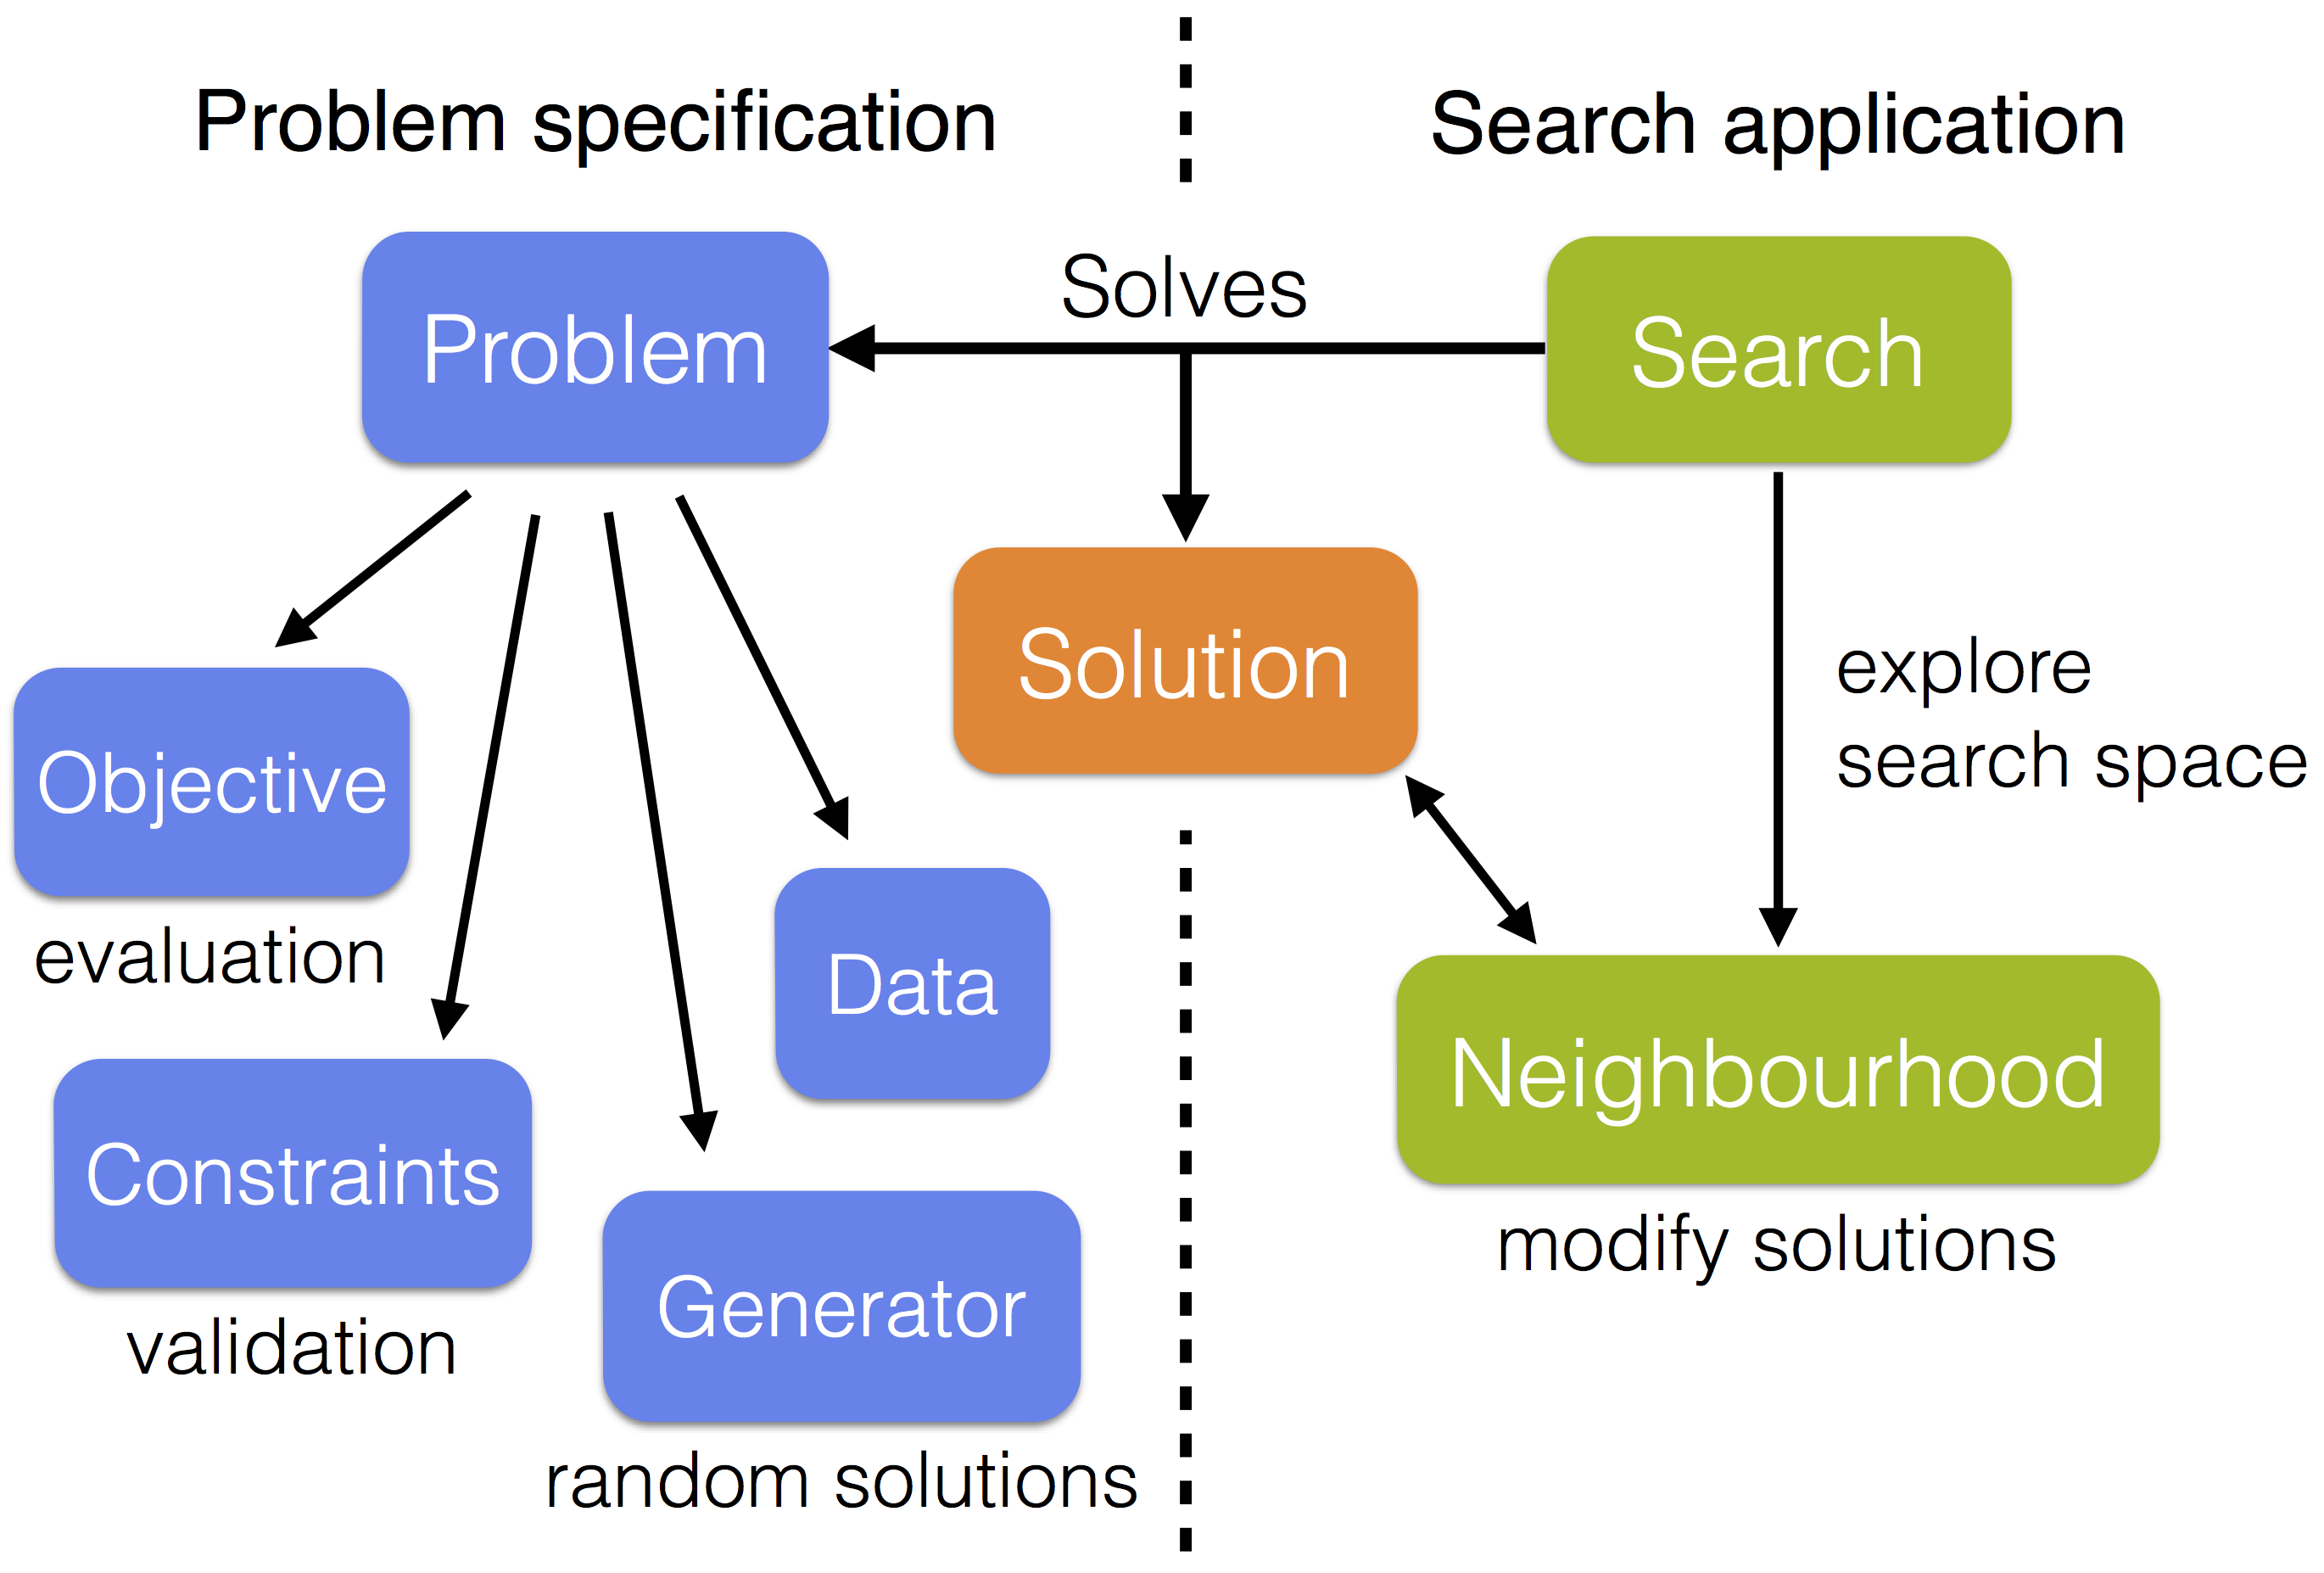
\includegraphics[scale=0.1]{images/diagram-detailed.png}
	\caption {
		 Diagram reprezentujący działanie biblioteki JAMES oraz elementy potrzebne do zdefiniowania problemu (źródło: \url{http://www.jamesframework.org/docs/})
	}
	\label{fig:james}
\end{figure}

Opis elementów biblioteki:
\begin{itemize}
    \item Solution - obiekt reprezentujący kompletne rozwiązanie problemu, który zawiera następujące dane
    \item Problem specification - specyfikacja problemu, która składa się z następujących elementów:
    \begin{itemize}
        \item Generator - obiekt służący do losowego generowania rozwiązań,
        \item Constraints - obiekty służace do walidacji rozwiązań pod względem spełniania stawianych warunków,
        \item Objective - obiekt służący do ewaluacji rozwiązania,
        \item Data - obiekt dostarczający przestrzeń rozwiązań.
    \end{itemize}
    \item Search application - zawiera następujące elementy:
    \begin{itemize}
        \item Search - znajduje się tutaj implementacja wybranego algorymu lokalnego przeszukiwania,
        \item Neighbourhood - obiekt umożliwiający modyfikacje rozwiązań w czasie działania algorytmu. Modyfikacje polegają na zmianie poszczególnych części rozwiązania na "sąsiednie".
    \end{itemize}
\end{itemize}

Biblioteka JAMES udostępnia szereg implementacji algorytmów metaheurystycznych służacych do lokalnego przeszukiwania przestrzeni rozwiązań w celu optymalizacji zadanego problemu. Wejściem każdego z algorytmów jest definicja problemu oraz kryterium stopu, które może być zdefiniowane jako maksymalny czas działania algorytmu bądź jako maksymalną liczbę kroków. W pracy zostały użyte następujące algorytmy pochodzące z tej biblioteki: Random Search, Random Descent, Steepest Descent, Tabu Search, Metropolis Search, Parallel Tempering.

\section{Dane opisujące właściwości żeliwa ADI}
\subsection{Zbieranie danych}
Dane na temat produkcji żeliwa ADI nie występują w sieci w postaci zagregowanej. Jedynymi źródłami, gdzie można je zdobyć, są artykuły oraz prace naukowe, w których autorzy podejmowali się badań nowych stopów i parametrów ich obróbki cieplnej. Rezultatami tych badań są w większości tabele przedstawiające jak dane składy wytopów oraz ich obróbka cieplna wpływały na właściwości mechaniczne. Część z artykułów, które zawierają bardzo obszerny przekrój różnych stopów i parametrów obróbki, przedstawia dane tylko w postaci wykresów, co wprowadza trudności w agregowaniu danych w jednym miejscu.

Zostało ustalone, że do zbioru danych będą zbierane następujące informacje:
\begin{itemize}
    \item skład chemiczny wytopu (zawartość procentowa pierwiastków):
    \begin{itemize}
        \item węgiel (C),
        \item krzem (Si),
        \item mangan (Mn),
        \item magnez (Mg),
        \item miedź (Cu),
        \item nikiel (Ni),
        \item molibden (Mo),
        \item siarka (S),
        \item fosfor (P),
        \item wanad (V),
        \item chrom (Cr).
    \end{itemize}
    \item ekwiwalent węglowy (CE) - obliczony jako\cite{joshi2020}: $CE = \%C+0.33(\%Si+\%P)$,
    \item parametry obróbki termicznej:    
    \begin{itemize}        
        \item temperatura i czas austenityzacji (aust\_temp, aust\_czas),       
        \item temperatura i czas ausferytyzacji (ausf\_temp, ausf\_czas).  
    \end{itemize}
    \item właściwości mechaniczne:    \begin{itemize}
        \item wytrzymałość na rozciąganie (Rm),
        \item granica plastyczności (Rp02),
        \item wydłużenie (A5),
        \item twardość,
        \item udarność.
    \end{itemize}
    \item grubość wytopu (mm),
    \item właściwości mechaniczne wytopu przed obróbką cieplną.
\end{itemize}

Budowa zbioru danych, który pozwoli na zbudowanie modeli predykcyjnych żeliwa ADI, okazała się procesem czasochłonnym. By lepiej zobrazować ten proces, zostały opracowane statystyki opisujące liczbę przeanalizowanych artykułów, zebranych rekordów, oraz rekordów odrzuconych na podstawie negatywnej oceny specjalistów.

Statystyki:
\begin{itemize}
    \item liczba zebranych artykułów/prac naukowych: 66,
    \item liczba zebranych rekordów (bez podziału na właściwości mechaniczne): 941 (w tym 252 rekordy odrzucone),
    \item liczba kompletnych rekordów (zawierających wszystkie właściwości mechaniczne, bez odrzuconych): 137,
    \item liczba zebranych rekordów (bez odrzuconych i z podziałem na właściwości mechaniczne): 1981,
    \item liczba unikalnych stopów: 94,
    \item liczba brakujących wartości: 1464 (42\% wszystkich możliwych wartości właściwości mechanicznych w zbiorze danych). 
\end{itemize}

Statystyka zebranych rekordów z podziałem na właściwości mechaniczne została przedstawiona na rysunku \ref{fig:stats}. Widać na nim, że dla dwóch właściwości mechanicznych (granica plastycznosci i udarność) liczbę zebranych danych w stosunku do wszystkich rekordów jest mniejsza niż 50\%. Dane te były najrzadziej występującymi w znalezionych pracach. Najczęściej występującymi danymi okazała się twardość, która była przestawiana w różnych skalach tj. skali twardości Brinella, skali twardości Rockwella oraz skali twardości Vickersa. Ze względu na większościowy udział danych przedstawionych w~postaci skali Brinella, dane w innych skalach zostały przekonwertowane do tej właśnie skali. Konwersja została przeprowadzona przy pomocy tabeli konwersji twardości \cite{hard_conversion}. Dodatkowym problemem okazała się udarność, gdyż także jest przedstawiana za pomocą dwóch różnych oznaczeń:
\begin{itemize}
    \item K - udarność mierzona na próbkach bez karbu,
    \item KV - udarność mierzona na próbkach z karbem V.
\end{itemize}
Ze względu na brak informacji o tym w jaki sposób te dwie wartości są ze sobą powiązane (brak danych opisujących jednocześnie udarność dla próbek z karbem oraz bez karbu), zostało założone, że $K = 11\cdot KV$ na podstawie tabel zawartych w normie PN-EN 1564:2012. Ze względu na większy udział rekordów zawierających udarność dla próbek bez karbu, rekordy z udarnością mierzoną na próbkach z karbem zostały przekonwertowane do wartości dla próbek bez karbu za pomocą wspomnianego wzoru.

\begin{figure}[ht]{}
	\centering
	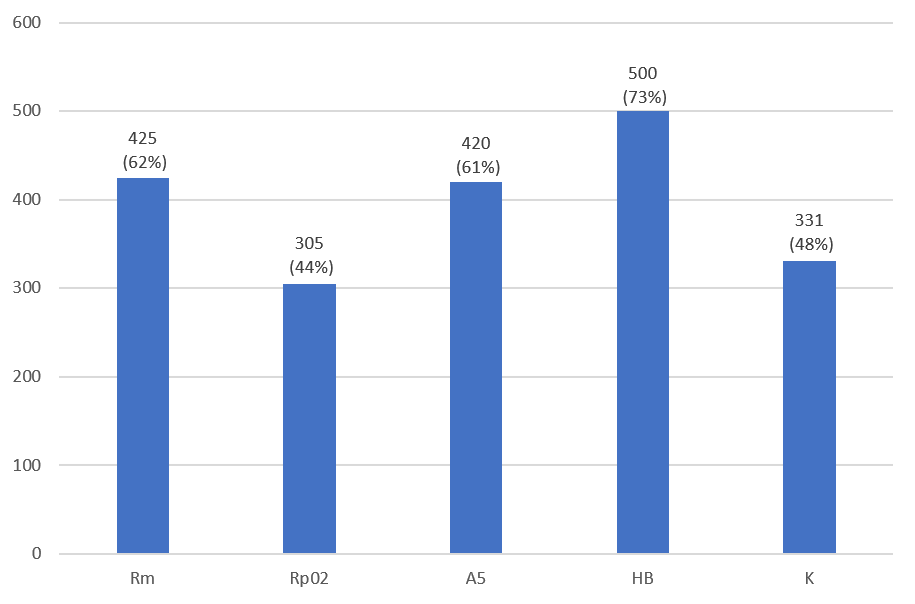
\includegraphics[scale=0.5]{images/statystyki.png}
	\caption {
		 Rozkład liczby zebranych danych dla każdej z właściwości mechanicznych.
	}
	\label{fig:stats}
\end{figure}

\subsection{Analiza zbioru danych}

W celu lepszego zrozumienia danych zostały sporządzone następujące graficzne reprezentacje:
\begin{itemize}
    \item wykresy pudełkowe - pozwalają na wskazanie wartości odstających,
    \item histogramy - pozwalają na wskazanie miejsc z brakującymi danymi,
    \item macierz korelacji - pozwala na określenie zależności między wymiarami.
\end{itemize}

Wykresy pudełkowe zostały sporządzone dla każdego z wymiarów i przedstawione w zagregowanej postaci na rysunkach \ref{fig:chem_box}, \ref{fig:heat_box} i \ref{fig:prop_thickness_box}. W przypadku wykresów dla składu chemicznego, w każdym wymiarze poza miedzią i niklem, wystepują wartości odstające. W~większości przypadków są to nieduże odstępstwa od średniej wartości w~danym wymiarze, więc można uznać, że są to mało pokryte zakresy wartości. Można jednak zauważyć wymiary, w których te odstępstwa są bardzo duże, co może wskazywać na błędy w~ artykułach, z których dane zostały zaczerpnięte. Przykładem może tutaj posłużyć wykres dla wymiaru fosforu, którego wartość średnia jest równa ok. 0,034, a największa wartość to 0,65, czyli 20 krotnie większa. Niestety, te odstępstwa nie zostały przeanalizowane przez ekspertów i przyjęte w badaniach jako poprawne. Dodatkową wadą wyrzucania wartości odstających w przypadku składu chemicznego byłoby wyrzucanie znacznej liczby rekordów ze zbioru, gdyż na każdy wytop przypada średnio ponad 9 rekordów.
\begin{figure}[ht]{}
	\centering
	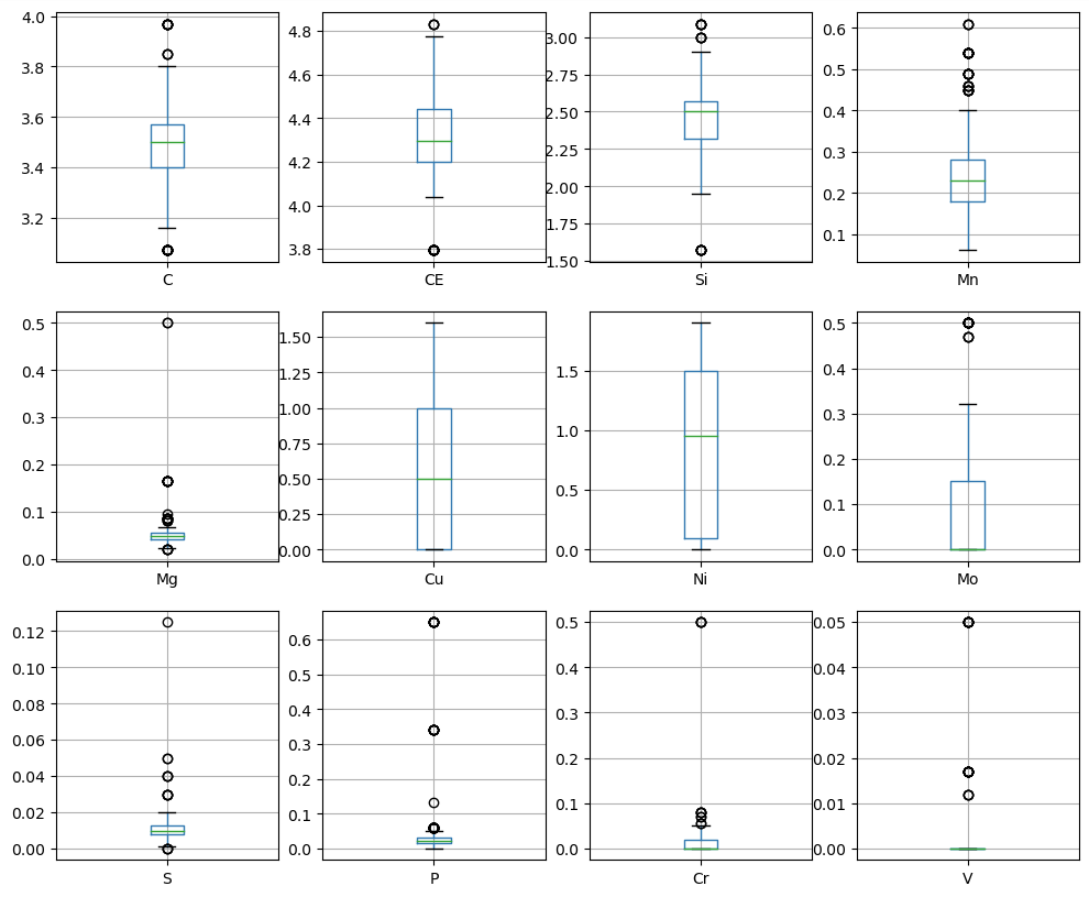
\includegraphics[scale=0.5]{images/chem_box.png}
	\caption {
		 Wykresy pudełkowe dla wymiarów składu chemicznego i ekwiwalentu węglowego.
	}
	\label{fig:chem_box}
\end{figure}

W przypadku wykresów dla wymiarów opisujących obróbkę termiczną, wymiarem rzucającym się w oczy jest temperatura austenityzacji. Wartość tego wymiaru oscyluje w okolicach wartości 900 stopni Celcjusza, gdyż jest to standardowa temperatura dla procesu austenityzacji. Wartości ukazane jako odstające, zostały celowo zostawione w zbiorze danych w celu zbadania jak inne wartości tej temperatury wpłyną na właściwości mechaniczne. Podobna sytuacja zachodzi w wymiarze opisującym temperaturę ausferrytyzacji - można zauważyć 3 wartości znacznie odstające od pozostałych danych lecz one także zostały zachowane w zbiorze danych.

\begin{figure}[ht]{}
	\centering
	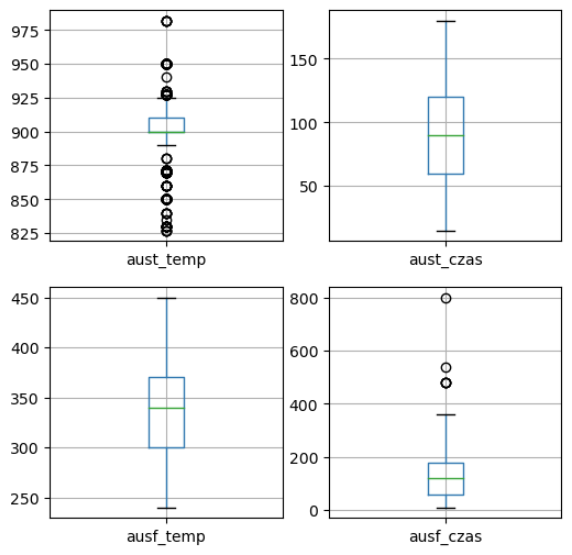
\includegraphics[scale=0.5]{images/heat_box.png}
	\caption {
		 Wykresy pudełkowe dla wymiarów obróbki termicznej.
	}
	\label{fig:heat_box}
\end{figure}

W przypadku wykresów dla właściwości mechanicznych oraz grubości, znacznie odstające dane można zauważyć w wymiarach K (udarność) oraz wymiarze opisującym grubość wytopu. Wartości odstające dla wymiaru udarności zostały pobrane z jednej pracy, która w sposób dokładny przedstawiła dane i nic nie wskazuje na to, by mogły być one niepoprawne. Dla wymiaru grubości wartości odstające wynikają z tego, że w większości prac badane były wytopy o grubości 25 mm.
\begin{figure}[ht]{}
	\centering
	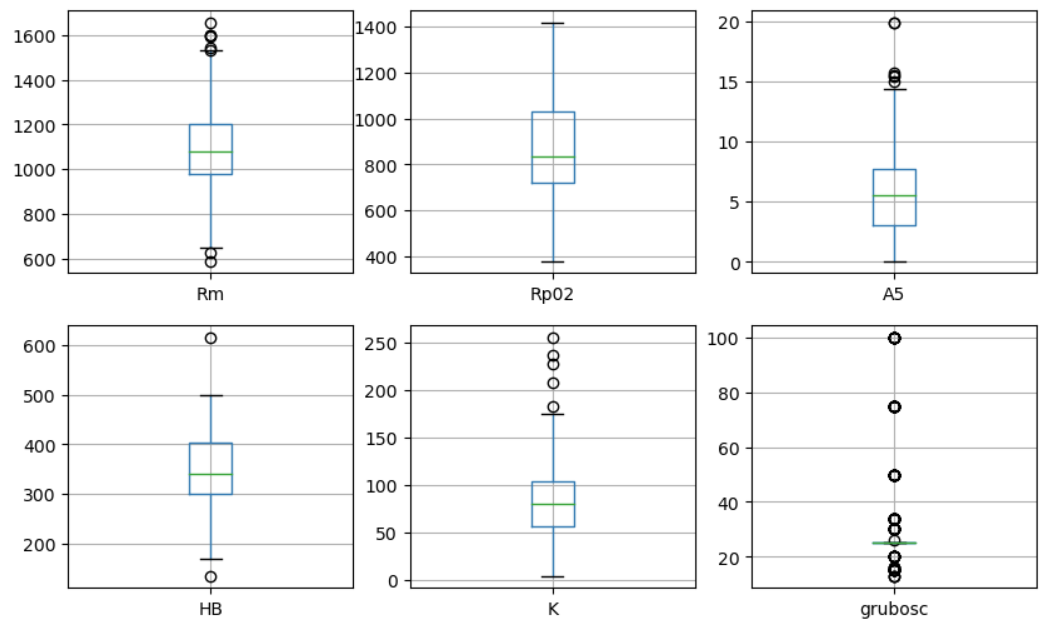
\includegraphics[scale=0.5]{images/prop_thickness_box.png}
	\caption {
		 Wykresy pudełkowe dla wymiarów właściwości mechanicznych oraz grubości wytopu.
	}
	\label{fig:prop_thickness_box}
\end{figure}

Histogramy zostały przedstawione na rys. \ref{fig:histogram}. Niektóre z nich są mało czytelne ze względu na znacznie odstające wartości. W przypadku wymiarów opisujących właściwości mechaniczne, histogramy pokazują, że rozkład każdego z nich ma kształt zbliżony do dzwonu oraz że w większości nie występują zakresy z brakującymi wartościami.
\begin{figure}[ht]{}
	\centering
	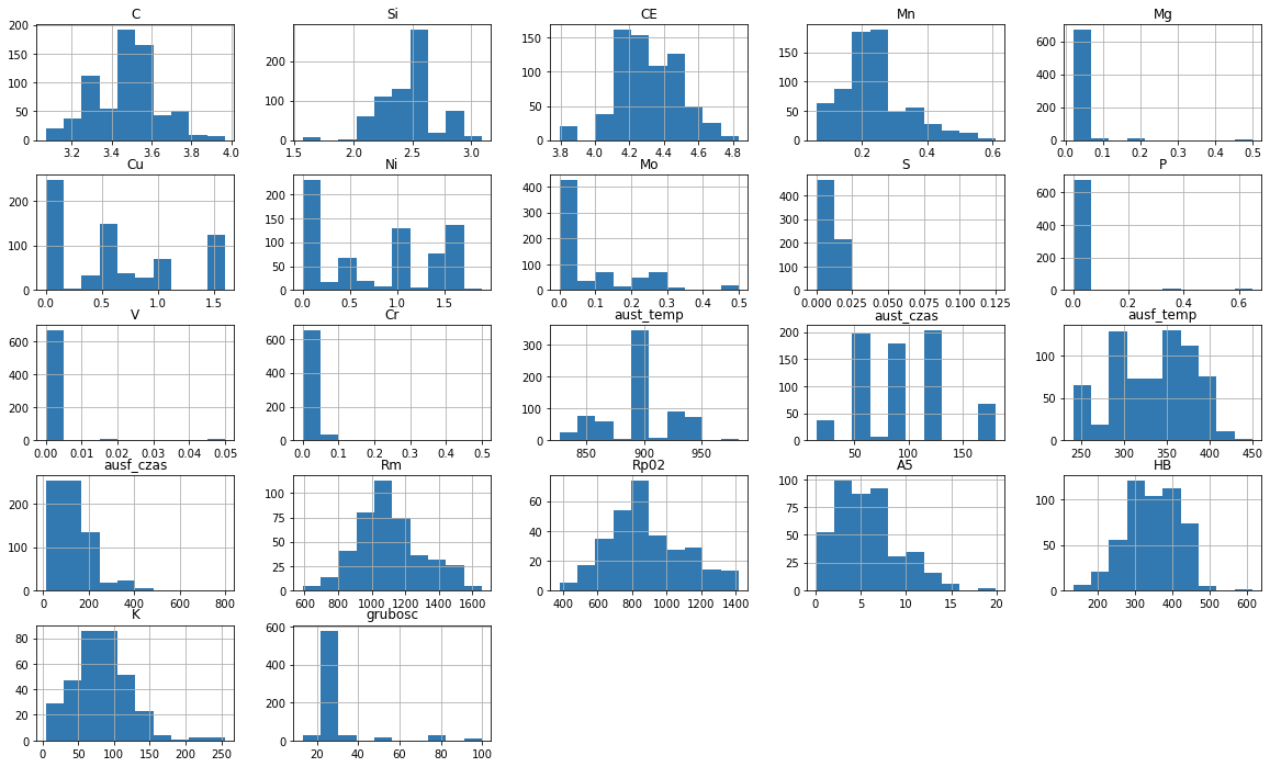
\includegraphics[scale=0.43]{images/histogram.png}
	\caption {
		 Histogramy dla wszystkich wymiarów w zbiorze danych.
	}
	\label{fig:histogram}
\end{figure}
\FloatBarrier
\subsection{Analiza korelacji zachodzących w zbiorze danych}\label{correlation-analysis}
\subsubsection{Macierz korelacji}
Macierz korelacji (rys. \ref{fig:correlation}) nie została przedstawiona dla wszystkich wymiarów ze względu na ich dużą liczbę oraz chęć zbadania korelacji między wymiarami opisującymi zależności miedzy procese produkcji i właściwościami mechanicznymi a właściwościami mechanicznymi. Widoczne w macierzy wartości są wartościami bezwględnymi w celu dostrzeżenia wymiarów najbardziej ze sobą skorelowanych. Macierz zostanie wykorzystana do analizy korelacji w zbiorze danych opisanej w punkcie \ref{correlation-analysis}.
\begin{figure}[ht]{}
	\centering
	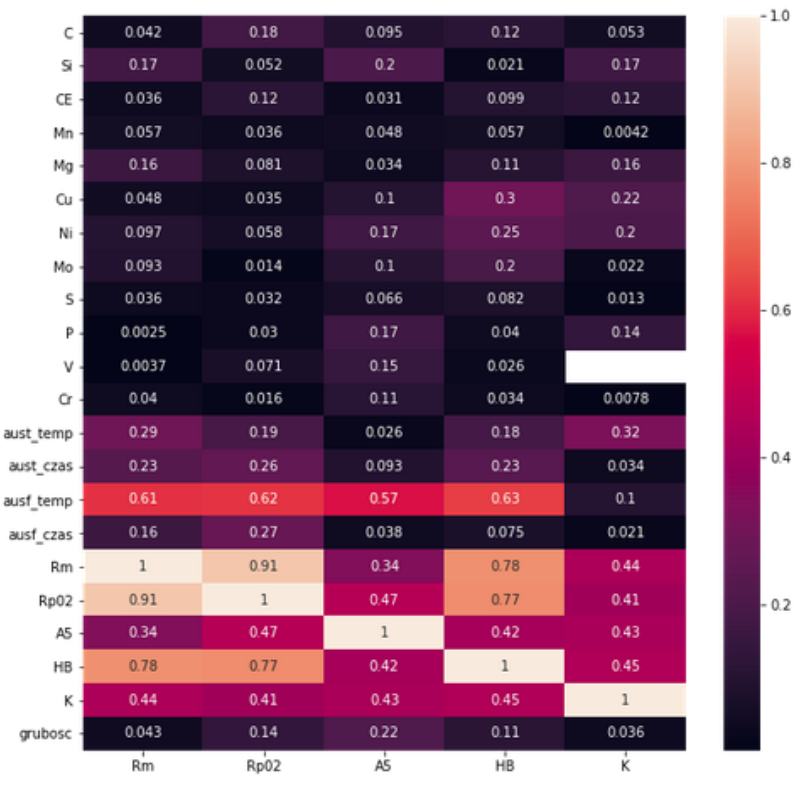
\includegraphics[scale=0.6]{images/correlation.png}
	\caption {
		 Macierz korelacji wszystkich wymiarów do wymiarów opisujących właściwości mechaniczne.
	}
	\label{fig:correlation}
\end{figure}
\FloatBarrier

\subsubsection{Analiza macierzy korelacji}
Przeprowadzona analiza powinna wskazać możliwość uzupełnienia brakujących danych wykorzystując inne wymiary, dla których wartości istnieją. 

Analizując macierz korelacji z rysunku \ref{fig:correlation}, można wyciągnąć następujące wnioski:
\begin{itemize}
    \item Zachodzi silna korelacja między wymiarami Rm oraz Rp02 (0.91),
    \item Wymiary Rm i Rp02 są także w znacznym stopniu skorelowane z wymiarem HB (0.78 i 0.77),
    \item Wymiar opisujący temperaturę ausferrytyzacji jest w pewnym stopniu skorelowany z wymiarami Rm, Rp02, A5, HB (ok. 0.6),
    \item Wymiar K opisujący udarność wygląda na słabo skorelowany z innymi wymiarami opisującymi właściwości fizyczne.
\end{itemize}

\subsubsection{Interpretacja wniosków do analizy korelacji}
Wnioski wyciągnięte podczas analizy korelacji pokazują w jasny sposób, że wymiary Rm, Rp02, A5, HB, ausf\_temp są ze sobą w znaczny sposób skorelowane i można założyć, że istnieje możliwość uzupełnienia brakujących danych w tych wymiarach wykorzystując inne istniejące już dane.
Ze względu na niski stopień korelacji wymiaru K do innych wymiarów, zostanie on pominięty na okres uzupełniania wyżej wymienionych wymiarów.

\subsection{Próba uzupełnienia brakujących danych}\label{sec:filling_data}

\subsubsection{Uproszczony sposób postępowania w celu uzupełnienia brakujących danych}
Problem brakujących danych został przedstawiony w pracy A. Kochańskiego pt. Knowledge in Imperfect Data \cite{Kochanski12}, gdzie zostało zaprezentowane przykładowe rozwiązanie. Mianowicie, w celu wypełnienia brakujących wartości należy znaleźć podzbiór próbek, w~ których dla wymiaru, w którym brakuje danych, istnieje wysoce skorelowany inny wymiar, na podstawie którego możliwe jest wyznaczenie brakującej wartości np. za pomocą regresji liniowej. W pracy stwierdzono, że zaletą takiego podejścia jest możliwość uzyskania nowych wartości granicznych zbioru danych. W przypadku, gdy korelacja między atrybutami nie występuje, brakująca wartość może zostać obliczona poprzez porównanie z~wybranymi rekordami ze zbioru zawierającego pełne dane.

\subsubsection{Przedstawienie metody uzupełniania brakujących danych}
Analizując przedstawiony powyżej uproszczony sposób postępowania w celu uzupełnienia brakujących danych, można wyciągnąć następujące założenia co do metody uzupełniania:
\begin{itemize}
    \item rozmiar podzbioru próbek powinien być określony, np. 10 próbek,
    \item może istnieć więcej niż jeden skorelowany wymiar, liczba takich wymiarów, która będzie brana pod uwagę powinna być określona, np. 2 wymiary,
    \item ze względu na duży rozrzut danych w zbiorze, podzbiór próbek powinien być wybrany w taki sposób, aby dane w wymiarach nieskorelowanych oraz niezwiązanych z właściwościami mechanicznymi żeliwa były dla siebie najbliższymi sąsiadami, 
    \item stosowanie regresji liniowej będzie adekwatne dla podzbiorów z bardzo wysokim współczynnikiem korelacji, tj. powyżej 0.8, dla podzbiorów z mniejszym współczynnikiem powinna zostać użyta inna metoda wyznaczania wartości (np. drzewa decyzyjne),
    \item im wyższy będzie współczynnik korelacji w danym podzbiorze oraz próbki z podzbioru będą w jak najmniejszej odległości od próbki, dla której będzie uzupełniana brakująca wartość, tym będzie bardziej prawdopodobne, że wyznaczona wartość będzie prawidłowa.
\end{itemize}

Dodatkowe założenia dotyczące metody uzupełniania:
\begin{itemize}
    \item ze względu na różną liczbę brakujących danych oraz różne stopnie skorelowania między wymiarami, w których istnieją brakujące dane, należy określić w jakiej kolejności wymiary będą uzupełnianie (np. na 3 pierwszych miejscach powinny się znajdować najliczniejsze wymiary, które są ze sobą mocno skorelowane - Rm, HB, Rp02),
    \item zakłada się, że uzupełnianie brakujących wartości może być realizowane z wykorzystaniem próbek, dla których wartości zostały uzupełnione we wcześniejszych etapach uzupełniania,
    \item korzystnym będzie uzupełnianie najpierw próbek, dla których w znalezionych podzbiorach jest wyższy współczynnik korelacji niż w pozostałych - w tym celu zakłada się, że na danym etapie uzupełniania danych będą uzupełniane tylko te próbki, dla których współczynnik korelacji dla podzbioru będzie wyższy lub równy progu, który będzie obowiązywał na danym etapie uzupełniania,
    \item ze względu na możliwość wykorzystania uzupełnionych danych przy uzupełnianiu innych, zakłada się, że proces uzupełniania dla konkretnego progu współczynnika korelacji będzie prowadzony dopóki istnieją próbki z podzbiorami spełniającymi dany próg (takie podejście pozwoli na wykorzystywanie próbek uzupełnionych w poprzednich krokach, które będą spełniały dany próg),
    \item ze względu na oczekiwane różne współczynniki korelacji w podzbiorach, zakłada się, że najpierw będą uzupełniane próbki z wysokimi współczynnikami korelacji wśród podzbiorów a następnie z mniejszymi,
    \item ze względu na to, że dla części danych znalezione podzbiory mogą mieć bardzo małe wartości korelacji, zakłada się ustalenie maksymalnej liczby etapów uzupełniania danych, po której proces uzupełniania zostanie przerwany.
\end{itemize}

Na podstawie powyższych założeń została sporządzona metoda uzupełniania brakujących wartości w zbiorze danych opisującym właściwości mechaniczne żeliwa ADI. 

W celu uzupełnienia brakujących danych należy ustalić:
\begin{itemize}
    \item kolejność uzupełnianych wymiarów,
    \item początkowy próg współczynnika korelacji (wspomniany w założeniach),
    \item liczba próbek w podzbiorze,
    \item granica współczynnika korelacji, do której stosowana będzie regresja liniowa,
    \item liczba wymiarów, na podstawie której przewidywana będzie brakująca wartość,
    \item algorytm uczenia maszynowego używany poza regresją liniową.
\end{itemize}

Metoda uzupełniania polega na znajdowaniu podzbioru próbek, które są najbliższymi sąsiadami uzupełnianej próbki dla wymiarów określonych jako nieskorelowane i nie będące związane z właściwościami fizycznymi żeliwa. Ustalanie brakującej wartości  polega na przewidywaniu jej wykorzystując model zbudowany z danych w znalezionym podzbiorze. W pierwszej kolejności uzupełniane są próbki, dla których średni współczynnik korelacji w~ ustalonym podzbiorze będzie przekraczał zadany próg. Próg wraz z brakiem zmiany liczby brakujących wartości, jest zmniejszany o ustaloną wartość np. 0.05. Próbki do ustalonej wartości współczynnika korelacji  w podzbiorze (np. 0.8) są uzupełniane za pomocą regresji liniowej, następnie wykorzystywany jest inny algorytm uczenia maszynowego np. drzewo decyzyjne. Dla danego progu współczynnika korelacji odbywa się pewna liczba kroków uzupełnienia brakujących wartości za sprawą wykorzystywania danych, które zostały uzupełnione we wcześniejszych krokach. Obniżenie progu następuje, gdy liczba brakujących danych się nie zmniejsza. Koniec uzupełniania następuje, gdy wszystkie brakujące wartości zostaną uzupełnione albo gdy liczba kroków przekroczy ustaloną maksymalną liczbę kroków.

\subsubsection{Pseudokod algorytmu}\label{sec:filling-pseudocode}
Pseudokod algorytmu został przedstawiony w trzech częściach, z których pierwsza (Algorytm \ref{algo:uzupelnianie}) przedstawia główne kroki algorytmu. 
Opis danych wejściowych alg. \ref{algo:uzupelnianie}:
\begin{itemize}
\item X - zbiór danych,
\item order - kolejność uzupełnianych wymiarów,
\item corr\_cutoff\_bound - początkowy próg korelacji,
\item req\_neighs - liczba próbek w podzbiorze, 
\item linear\_reg\_to - granica współczynnika korelacji, do której stosowana będzie regresja liniowa,
\item amount\_of\_feats\_to\_predict - liczba wymiarów, na podstawie której przewidywana jest brakująca wartość,
\item max\_steps - maksymalna liczba kroków,
\item next\_predictor\_provider - obiekt służący do zwracania algorytmu uczenia maszynowego używanego po przekroczeniu granicy używania regresji liniowej.
\end{itemize}
Wynik: zbiór danych uzupełniony w wymiarach określonych przez daną order.


Opis użytych funkcji pomocniczych i bardziej złożonych linii kodu w algorytmie \ref{algo:uzupelnianie}:
\begin{itemize}
    \item linia 2 - funkcja \textit{get\_missing\_values\_count}  przyjmująca zbiór próbek i zwracająca łączną liczbę brakujących wartości w wymiarach Rm, Rp02, HB, A5, K,
    \item linia 10 - wywołanie procedury \textit{fill\_missing} opisanej w algorytmie \ref{algo:fillMissing}
\end{itemize}

\begin{algorithm}[ht]
\DontPrintSemicolon
  \KwInput{order, corr\_cutoff\_bound, req\_neighs, linear\_reg\_to, amount\_of\_feats\_to\_predict, max\_steps, next\_predictor\_provider}
  \KwOutput{wypełniony zbiór próbek X}
  \SetKw{Continue}{continue}
  \KwData{zbiór próbek X}
  \SetKwFunction{getMissingValuesCount}{get\_missing\_values\_count}
  \SetKwFunction{getFeaturesWithNulls}{get\_features\_with\_nulls}
  \SetKwFunction{getCorrelationMatrix}{get\_correlation\_matrix}
  \SetKwFunction{mostCorrelatedFeaturesExceptNullFeatures}{most\_corr\_feats}
  \SetKwFunction{removeFeatsWithNulls}{remove\_features\_with\_nulls}
  \SetKwFunction{minMaxScaler}{min\_max\_scaler}
  \SetKwFunction{findNearestNeighs}{find\_nearest\_neighs}
  \SetKwFunction{fillMissing}{fill\_missing}
  \SetKwData{CorrCutoff}{corr\_cutoff}
  \SetKwData{MissingValuesCount}{missing\_values\_count}
  \SetKwData{Filled}{filled} 
  \SetKwData{NullFeatures}{null\_features} 
  \SetKwData{Correlated}{correlated} 
  \SetKwData{CorrelationMatrix}{corr\_matrix}
  \SetKwData{NotCorrelated}{not\_correlated}
  \SetKwData{Xprim}{X'}
  \SetKwData{Scaler}{scaler}
  \SetKwData{Neighs}{neighs}
  \SetKwData{NearestNeighs}{nearest\_neighbors}
  \SetKwData{Step}{step}
  \SetKwData{ActuallyMissing}{actually\_missing}

  $\CorrCutoff \leftarrow corr\_cutoff\_bound $\;
  $\MissingValuesCount \leftarrow \getMissingValuesCount(X) $\;
  \Repeat{\Filled == size(order) or step == max\_steps}{
    $\Filled \leftarrow 0 $\;
    \For{feature in order}{
        \If{all values for feature are filled}{
            $\Filled \leftarrow \Filled + 1 $\;
            \Continue
        }
        \For{row in X}{
            \tcp{procedura \fillMissing została zdefiniowana w algorytmie \ref{algo:fillMissing}}
            $\fillMissing(row, feature, amount\_of\_feats\_to\_predict, req\_neighs, \newline \hspace*{6em}corr\_cutoff, linear\_reg\_to, next\_predictor\_provider)$\;
        }
        $\Step \leftarrow \Step + 1$\;
        $\ActuallyMissing \leftarrow \getMissingValuesCount(X)$\;
        \If{\MissingValuesCount == \ActuallyMissing}{
            $corr\_cutoff \leftarrow corr\_cutoff - 0.05$\;
        }
        $\MissingValuesCount \leftarrow \ActuallyMissing $\;
    }
  }
  \KwRet{X}
  
    \caption{Uzupełnianie zbioru danych}\label{algo:uzupelnianie}
\end{algorithm}

\FloatBarrier

Opis danych wejściowych procedury \textit{fill\_missing} (alg. \ref{algo:fillMissing}):
\begin{itemize}
    \item row - wiersz ze zbioru próbek X, w którym będzie uzupełniana brakująca wartość,
    \item feature - nazwa aktualnie uzupełnianego wymiaru (np. Rm),
    \item amount\_of\_feats\_to\_predict - opisane dla alg. \ref{algo:uzupelnianie},
    \item req\_neighs - opisane dla alg. \ref{algo:uzupelnianie},
    \item corr\_cutoff - aktualny próg wartości współczynnika korelacji,
    \item linear\_reg\_to - opisane dla alg. \ref{algo:uzupelnianie},
    \item next\_predictor\_provider - opisane dla alg. \ref{algo:uzupelnianie}.
\end{itemize}

Opis użytych funkcji pomocniczych i bardziej złożonych linii kodu w algorytmie \ref{algo:fillMissing}:
\begin{itemize}
    \item linia 4 - funkcja \textit{get\_features\_with\_null} przyjmująca aktualnie rozpatrywany wiersz i zwracająca zbiór wszystkich wymiarów z tego wiersza, w których brakuje wartości,
    \item linia 7 - funkcja \textit{most\_corr\_feats} przyjmująca wartości współczynników korelacji do rozpatrywanego wymiaru (feature), stałą \textit{amounts\_of\_feats\_to\_predict} oraz zbiór wymiarów z brakującymi wartościami i zwracająca n najbardziej skorelowanych wymiarów do rozpatrywanego wymiaru (feature), gdzie n jest równe \textit{amounts\_of\_feats\_to\_predict},
    \item linia 11 - funkcja \textit{remove\_features\_with\_nulls} przyjmująca zbiór próbek X oraz zbiór wymiarów \textit{not\_correlated} i zwracająca zbiór wymiarów \textit{not\_correlated} z usuniętymi wymiarami, w których brakuje wartości,
    \item linia 13 i 14 - funkcja \textit{min\_max\_scaler} zwracająca obiekt skalera i przy wywołaniu funkcji \textit{scale} na tym obiekcie, zwraca zbiór próbek X' przeskalowany do wartości [-1, 1],
    \item linia 15 - nadpisanie składowej \textit{feature} wiersza ze zbioru próbek \textit{row} wartością zwróconą przez funkcję \textit{predict\_value}, która została przedstawiona w algorytmie \ref{algo:predictValue}.
\end{itemize}


\begin{algorithm}
    \caption{Procedura uzupełniania wartości brakującej w danej próbce}
    \label{algo:fillMissing}
    \DontPrintSemicolon
    
    \SetKw{Continue}{continue}
    \SetKwFunction{getMissingValuesCount}{get\_missing\_values\_count}
    \SetKwFunction{getFeaturesWithNulls}{get\_features\_with\_nulls}
    \SetKwFunction{getCorrelationMatrix}{get\_correlation\_matrix}
    \SetKwFunction{mostCorrelatedFeaturesExceptNullFeatures}{most\_corr\_feats}
    \SetKwFunction{removeFeatsWithNulls}{remove\_features\_with\_nulls}
    \SetKwFunction{minMaxScaler}{min\_max\_scaler}
    \SetKwFunction{findNearestNeighs}{find\_nearest\_neighs}
    \SetKwFunction{PredictValue}{predict\_value}
    \SetKwData{CorrCutoff}{corr\_cutoff}
    \SetKwData{MissingValuesCount}{missing\_values\_count}
    \SetKwData{Filled}{filled} 
    \SetKwData{NullFeatures}{null\_features} 
    \SetKwData{Correlated}{correlated} 
    \SetKwData{CorrelationMatrix}{corr\_matrix}
    \SetKwData{NotCorrelated}{not\_correlated}
    \SetKwData{Xprim}{X'}
    \SetKwData{Scaler}{scaler}
    \SetKwData{Neighs}{neighs}
    \SetKwData{NearestNeighs}{nearest\_neighbors}
    \SetKwProg{Proc}{Procedure}{ is}{end}
    \SetKwFunction{FillMissing}{fill\_missing}
    \Proc{\FillMissing{row, feature, amount\_of\_feats\_to\_predict, req\_neighs, corr\_cutoff, linear\_reg\_to, next\_predictor\_provider}}{
        \KwData{zbiór próbek X}
        \If{row[feature] is not null}{
                \Continue
            }
        $\NullFeatures \leftarrow \getFeaturesWithNulls(row) $\;
        $\NullFeatures.remove(feature) $\;
        $\CorrelationMatrix \leftarrow \getCorrelationMatrix(X) $\;
        $\Correlated \leftarrow \mostCorrelatedFeaturesExceptNullFeatures(\CorrelationMatrix[feature], \newline \hspace*{13em} amount\_of\_feats\_to\_predict, \newline
        \hspace*{13em} \NullFeatures)$\;
        $\Correlated.remove(feature)$\;
        $\NotCorrelated \leftarrow X.features - \Correlated$\;
        $\NotCorrelated.remove(feature)$\;
        $\NotCorrelated \leftarrow \removeFeatsWithNulls(X, \NotCorrelated)$\;
        $\Xprim \leftarrow X[\NotCorrelated]$\;
        $\Scaler \leftarrow \minMaxScaler(\Xprim)$\;
        $\Xprim \leftarrow \Scaler.scale(\Xprim)$\;
        \tcp{Funkcja \PredictValue została zdefiniowana w algorytmie \ref{algo:predictValue}}
        $row[feature] \leftarrow \PredictValue(\Xprim, \NotCorrelated, \Correlated, \Scaler, req\_neighs, \newline \hspace*{13em}amount\_of\_feats\_to\_predict, corr\_cutoff, \newline 
        \hspace*{13em}linear\_reg\_to, next\_predictor\_provider)$\;
    }
\end{algorithm}

\FloatBarrier
Opis danych wejściowych funkcji \textit{predict\_value} (alg. \ref{algo:predictValue}):
\begin{itemize}
    \item X' - zbiór przeskalowanych próbek zawierający wymiary nieskorelowane,
    \item not\_correlated - zbiór wymiarów nieskorelowanych,
    \item correlated - zbiór wymiarów skorelowanych,
    \item scaler - obiekt umożliwiający skalowanie wartości do zakresu [-1,1],
    \item req\_neighs - opisane dla alg. \ref{algo:uzupelnianie},
    \item amount\_of\_feats\_to\_predict - opisane dla alg. \ref{algo:uzupelnianie},
    \item corr\_cutoff - aktualny próg wartości współczynnika korelacji,
    \item next\_predictor\_provider - opisane dla alg. \ref{algo:uzupelnianie},
    \item linear\_reg\_to - opisane dla alg. \ref{algo:uzupelnianie}.
\end{itemize}

Opis użytych funkcji pomocniczych i bardziej złożonych linii kodu w algorytmie \ref{algo:predictValue}:
\begin{itemize}
    \item linia 4 - funkcja \textit{find\_nearest\_neighs} przymująca zbiór X', przeskalowany wektor wartości z wiersza\ textit{row} dla zbioru wymiarów \textit{not\_correlated} oraz liczba sąsiadów do znalezienia,
    \item linia 5 - funkcja \textit{remove\_neighs\_with\_nulls} przyjmująca zbiór najbliższych sąsiadów \textit{nns} i zbiór wymiarów skorelowanych \textit{correlated} i zwracająca tylko tych sąsiadów, dla których istnieją wartości we wszystkich skorelowanych wymiarach,
    \item linia 9 - funkcja \textit{features\_above\_corr\_cutoff} przyjmująca wektor współczynników korelacji dla wymiaru \textit{feature} pochodzący z macierzy korelacji \textit{corr\_matrix}, stałą \textit{amount\_of\_feats\_to\_predict} oraz stałą \textit{ corr\_cutoff} i zwracająca n najbardziej skorelowanych wymiarów, które spełniają warunek współczynnika korelacji większego lub równego \textit{corr\_cutoff} ( n - \textit{amount\_of\_feats\_to\_predict}).
\end{itemize}

\begin{algorithm}
    \DontPrintSemicolon
    
    \SetKw{Continue}{continue}
    \SetKwFunction{getMissingValuesCount}{get\_missing\_values\_count}
    \SetKwFunction{getFeaturesWithNulls}{get\_features\_with\_nulls}
    \SetKwFunction{getCorrelationMatrix}{get\_correlation\_matrix}
    \SetKwFunction{mostCorrelatedFeaturesExceptNullFeatures}{most\_corr\_feats}
    \SetKwFunction{removeFeatsWithNulls}{remove\_features\_with\_nulls}
    \SetKwFunction{minMaxScaler}{min\_max\_scaler}
    \SetKwFunction{findNearestNeighs}{find\_nearest\_neighs}
    \SetKwFunction{removeNeighsWithNulls}{remove\_neighs\_with\_nulls}
    \SetKwFunction{getFeatsAboveCorrCutoff}{features\_above\_corr\_cutoff}
    \SetKwData{CorrCutoff}{corr\_cutoff}
    \SetKwData{MissingValuesCount}{missing\_values\_count}
    \SetKwData{Filled}{filled} 
    \SetKwData{Predictor}{predictor} 
    \SetKwData{NullFeatures}{null\_features} 
    \SetKwData{Correlated}{correlated} 
    \SetKwData{CorrelationMatrix}{corr\_matrix}
    \SetKwData{NotCorrelated}{not\_correlated}
    \SetKwData{Xprim}{X'}
    \SetKwData{Neighs}{neighs}
    \SetKwData{NearestNeighs}{nns}
    \SetKwData{PredictedValue}{predicted\_value}
    \SetKwProg{Fn}{Function}{ is}{end}
    \SetKwFunction{PredictValue}{predict\_value}
    \Fn{\PredictValue{X’, not\_correlated, correlated, scaler, req\_neighs, amount\_of\_feats\_to\_predict, corr\_cutoff, linear\_reg\_to, next\_predictor\_provider}}{
        \KwResult{Przewidziana wartość}
        $\Neighs \leftarrow req\_neighs$\;
        \Repeat{size(\NearestNeighs) >= req\_neighs}{
            $\NearestNeighs \leftarrow \findNearestNeighs(\Xprim, scaler.scale(row[\NotCorrelated]), \Neighs)$\;
            $\NearestNeighs \leftarrow \removeNeighsWithNulls(\NearestNeighs, correlated)$\;
            $\Neighs \leftarrow \Neighs + (req\_neighs - size(\NearestNeighs))$\;
        }
        $\CorrelationMatrix \leftarrow \getCorrelationMatrix(\NearestNeighs) $\;
        $correlated \leftarrow \getFeatsAboveCorrCutoff(\CorrelationMatrix[feature], \newline \hspace*{13em}amount\_of\_feats\_to\_predict, corr\_cutoff)$\;
        \If{size(correlated) == 0}{
            \KwRet{null}
        }
        \If{corr\_cutoff >= linear\_reg\_to}{
            $\Predictor \leftarrow LinearRegression()$\;
        }
        \Else{
            $\Predictor \leftarrow next\_predictor\_provider.provide()$\;
        }
        $\Predictor.train(\NearestNeighs[correlated], \NearestNeighs[feature])$\;
        $\PredictedValue \leftarrow \Predictor.predict(row[correlated])$\;
        \If{\PredictedValue > 0}{\KwRet{\PredictedValue}}
        \Else{\KwRet{null}}
    }
    \caption{Funkcja przewidująca wartość służącą do uzupełniania próbki}
    \label{algo:predictValue}
\end{algorithm}

\FloatBarrier

\subsubsection{Implementacja algorytmu}
Algorytm został zaimplementowany przy użyciu narzędzi opisanych w sekcji \ref{sec:tools-data-analysis-modeling}. Implementacja opisanego algorytmu została wzbogacona o zbieranie informacji o~ sposobie uzupełniania brakujących danych:
\begin{itemize}
    \item wymiary służące do zbudowania podzbioru tzw. sąsiadów próbki,
    \item wymiary wybrane jako skorelowane w podzbiorze na podstawie których jest budowany model do przewidywania,
    \item współczynniki korelacji powyżej wspomnianych wymiarów do wymiaru, w którym była obecna brakująca wartość,
    \item wartość minimalna i maksymalna wymiaru z brakującą daną  w podzbiorze sąsiadów,
    \item indeksy próbek z podzbioru sąsiadów, które zostały wybrane do zbudowania modelu,
    \item numer kroku, w którym brakująca wartość została przewidziana.
\end{itemize}

\section{Budowa modeli predykcyjnych}\label{sec:model-realization}
Jak zostało już wspomniane w sekcji \ref{sec:model}, zachodzi potrzeba zbudowania modelu, który będzie reprezentował przestrzeń rozwiązań problemu opisanego w sekcji \ref{sec:problemDescription}. Nie było jednak możliwe zbudowanie wspólnego modelu dla wszystkich właściwości mechanicznych ze względu na podjęcię się tej części realizacji przed ukończeniem procesu uzupełniania danych, które nie przebiegło zgodnie z planem. 
Dla każdej z właściwości mechanicznych zostały zbudowane niezależne modele przy użyciu różnych zbiorów danych, które posiadały części wspólne ze względu na obecność rekordów o wszystkich właściwościach.

Do budowy takich modeli z powodzeniem stosowane są algorytmy uczenia maszynowego. W rozpatrywanym przypadku zostały wykorzystane modele regresyjne, które modelują związki pomiędzy dwiema lub więcej zmiennymi. Użyte algorytmy oraz narzędzia zostały opisane w sekcji \ref{sec:tools-data-analysis-modeling}.

\subsection{Redukcja wymiarowości zbioru, normalizacja i wymiar dogenerowany}
Ze względu na brak szczegółowej wiedzy na temat relacji między parametrami składu chemicznego a właściwościami mechanicznymi, przy redukcji wymiarowości została wzięta pod uwagę porada ekspertów. Zbiór danych został zredukowany o wymiary S, P, V, Cr ze względu na brak wpływu na właściwości mechaniczne oraz bardzo małą liczbę danych różnych od 0 w przypadku wymiarów Cr i V.

Wymiary wejściowe zostały znormalizowane metodą min-max do zakresu [-0.5;0.5]. Normalizacja została dokonana przy użyciu narzędzia MinMaxScaler z biblioteki scikit-learn. Warto tutaj wspomnieć, że normalizacja została dokonana na całym zbiorze danych przed podziałem na podzbiory dla właściwości mechanicznych.

Zbiór danych został rozszerzony o nowy wymiar, który przedstawia czas ausferrytyzacji przedstawiony w sekundach za pomocą logarytmu dziesiętnego. Takie rozszerzenie zbioru danych zostało zaproponowane w pracy M. A. Yescasa \cite{YESCAS2001162}, gdzie powołuje się on na swoją poprzednią pracę, w której dostrzegł, że taka forma lepiej opisuje czas ausferrytyzacji.

\subsection{Budowa zbioru treningowego i testowego}\label{sec:dataset}
Ze względu na małą liczbę próbek (689) w stosunku do liczby wymiarów (14) nie jest możliwe wyciągnięcie losowego zbioru próbek przeznaczonych na zbiór testowy bez utraty istotnych informacji ze zbioru treningowego. Aby temu zapobiec, została wykorzystana 5-krotna walidacja krzyżowa z zachowaniem takiego samego udziału próbek z każdej klasy. Ze względu na to, że wymiarami wyjściowymi są liczby, zostało stworzone 5 klas (1, 2, 3, 4, 5), które dzielą wartości na 5 zbiorów zbliżonych do siebie rozmiarem, poprzez ustalenie zakresu wartości wchodzących w skład danego zbioru. Liczność zbiorów reprezentujących klasy została przedstawiona na rys. \ref{fig:bins}. Zakresy wartości dla poszczególnych klas dla każdej z właściwości mechanicznych były następujące:
\begin{itemize}
    \item Rm: 1 - [Rm$_{min}$, 960), 2 - [960, 1045), 3 - [1045, 1127), 4 - [1127, 1264), 5 - [1264, Rm$_{max}$],
    \item Rp02: 1 - [Rp02$_{min}$, 696), 2 - [696, 813), 3 - [813, 900), 4 - [900, 1100), 5 - [1100, Rp02$_{max}$],
    \item HB : 1 - [HB$_{min}$, 286), 2 - [286, 325), 3 - [325, 370), 4 - [370, 415), 5 - [415, HB$_{max}$],
    \item A5 : 1 - [A5$_{min}$, 2.7), 2 - [2.7, 4.5), 3 - [4.5, 6.5), 4 - [6.5, 8.4), 5 - [8.4, A5],
    \item K : 1 - [K$_{min}$, 52), 2 - [52, 75), 3 - [75, 90), 4 - [90, 110), 5 - [110, K$_{max}$]
\end{itemize}

\begin{figure}[ht]{}
	\centering
	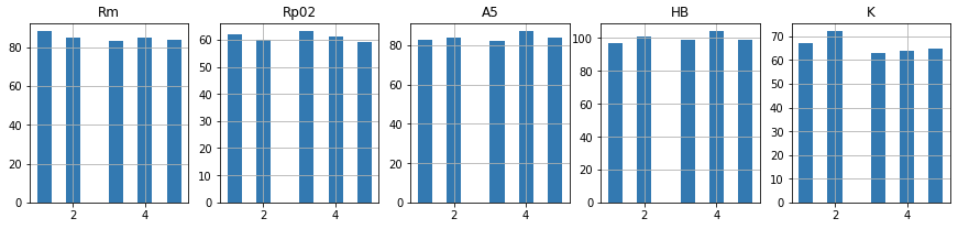
\includegraphics[scale=0.6]{images/bins.png}
	\caption {
		 Liczności zbiorów reprezentujących klasy, które rozdzielają wartości w wymiarach wyjściowych modeli.
	}
	\label{fig:bins}
\end{figure}
\FloatBarrier

\subsection{Trenowanie modeli}
Proces trenowania modeli został przeprowadzony w następujący sposób:
\begin{itemize}
    \item trenowanie każdego z modeli zostało przeprowadzone z wykorzystaniem walidacji krzyżowej wspomnianej w punkcie \ref{sec:dataset},
    \item dla każdego z algorytmów zostały wybrane różne wartości parametrów sterujących ich działaniem
    \item tuning parametrów został przeprowadzony poprzez trenowanie modeli dla każdej permutacji parametrów algorytmu,
    \item metryki użyte w celu oceny jakości wytrenowanych modeli: \begin{itemize}
        \item MAE (mean absolute error) - średni błąd bezwzględny,
        \item $R^{2}$ - współczynnik determinacji,
    \end{itemize}
    \item model po ewaluacji metryk jest douczany na zbiorze testowym,
    \item do badań porównawczych zostały wykorzystane po jednym najlepszym modelu dla każdej z metryk (sekcja \ref{sec:comp-eval}).
\end{itemize}

\subsubsection{Trenowanie modeli z wykorzystaniem algorytmu Random Forest} \label{sec:rf-train}
Algorytm Random Forest w przypadku implementacji pochodzącej z biblioteki scikit-learn posiada wiele parametrów, które wpływają na jego działanie. W celu znalezienia najlepszych modeli, zostały przetestowane następujące parametry:
\begin{itemize}
    \item n\_estimators - liczba drzew w lesie,
    \item max\_depth - maksymalna głębokość drzew,
    \item max\_features - liczba wymiarów rozpatrywanych przy szukaniu najlepszego podziału,
    \item criterion - metryka służąca do pomiaru jakości podziału,
    \item min\_samples\_split - minimalna liczba próbek potrzebna do podzielenia węzła w~ drzewie.
\end{itemize}
\subsubsection{Trenowanie modeli z wykorzystaniem algorytmu Gradient Boosting}\label{sec:gb-train}
Trenowanie modeli z użyciem algorytmu Gradient Boosting zostało przeprowadzone w identyczny sposób jak w przypadku trenowania modeli z użyciem algorytmu Random Forest.

Parametry algorytmu użyte podczas badań:
\begin{itemize}
    \item learning\_rate,
    \item subsample - współczynnik określający jaka część próbek treningowych zostanie losowo wybrana do trenowania przed rozrastaniem się drzew,
    \item max\_depth - maksymalna głębokość drzewa,
    \item eval\_metric - metryka służąca do ewaluacji modelu,
    \item booster - rodzaj używanego boostera.
\end{itemize}

Kombinacja wszystkich możliwych parametrów tworzy 216 unikalnych zbiorów. Podobnie jak w poprzednim algorytmie, parametr random\_state był ustawiony z jedną wartością dla każdego procesu uczenia.

W celu zbadania przestrzeni parametrów ponownie zostało zastosowane narzędzie GridSearchCV. Czas potrzebny na wytrenowanie wszystkich modeli wyniósł 10 sekund.

\subsubsection{Trenowanie modeli z wykorzystaniem algorytmu Multilayer Perceptron}\label{sec:mlp-train}
Do tworzenia i trenowania modeli z wykorzystaniem algorytmu Multilayer Perceptron został wykorzystany interfejs Keras z biblioteki TensorFlow. Pozwala on na czytelne i~proste definiowanie architektury sieci neuronowej poprzez tworzenie modelu sekwencyjnego, do którego dodajemy kolejne warstwy sieci. Taki model jest ostatecznie kompilowany z użyciem wskazanej metody stochastycznego spadku wzdłuż gradientu oraz funkcją straty.

Tworzone modele sieci neuronowych składają się z trzech warstw sieci:
\begin{itemize}
    \item warstwa wejściowa z 14 neuronami,
    \item warstwa ukryta, dla której zostały zbadane następujące parametry i ich wartości:
    \begin{itemize}
        \item funkcja aktywacji: tangens hiperboliczny,
        \item regularyzacja L2 dla wag, biasów oraz wyjścia warstwy,
    \end{itemize}
    \item warstwa wyjściowa z jednym neuronem.
\end{itemize}
Modele kompilowane są przy użyciu optymalizatora Adam z parametrem 'learning\_rate' ustawionym na wartość 0.1 oraz funkcją straty zdefiniowaną jako błąd średniokwadratowy.

Proces uczenia został przeprowadzony z użyciem metody Early Stopping, która pozwala zapobiegać przeuczeniu się sieci poprzez sprawdzanie, czy wartość funkcji straty dla próbek walidacyjnych zmienia się trakcie procesu uczenia. 

\subsubsection{Trenowanie modeli z wykorzystaniem algorytmu Ensemble averaging}\label{sec:ea-train}
Budowa modelu z wykorzystaniem tego algorytmu została zaczerpnięta z pracy Miguela Yescasa \cite{YESCAS2001162}, gdzie autor w swojej pracy nazwał go modelem komitetu sieci neuronowych. Więcej informacji na temat tej pracy znajduje się w sekcji \ref{sec:sota-prediction}.

Algorytm Ensemble averaging polega na stworzeniu wielu modeli o różnych parametrach i połączeniu ich w jeden model w taki sposób, by wejście i wyjście takiego modelu nie różniło się niczym od pojedyńczego modelu. Wyjście modeli jest połączone i ostateczne wyjście modelu jest średnią wartością wyjść modeli wchodzących w skład komitetu.

Modele wchodzące w skład komitetu sieci zostały wytrenowane z różnymi stałymi regularyzacji oraz różnymi liczbami neuronów wchodzących w skład warstwy ukrytej. By ograniczyć liczbę różnych stałych regularyzacji, zostało przeprowadzone badanie mające na celu sprawdzić, które stałe będą się najlepiej spisywać dla modeli z 10 oraz 25 neuronami w warstwie ukrytej. 

Zbadanymi stałymi dla wag, biasów oraz wyjść warstwy były wartości:  [1e-1, 1e-2, 1e-3, 1e-4, 1e-5]. Badanie zostało przeprowadzone z użyciem 5-krotnej walidacji krzyżowej wraz ze zbieraniem wartości metryk $R^{2}$ i średniego błędu absolutnego. Analiza badań opisana w punkcie \ref{sec:ea-eval} dostarczyła wartości stałych, które zostały przedstawione w tabeli \ref{tab:regularization}.
\begin{table}
\caption{Najlepsze stałe regularyzacji względem metryki $R^{2}$ dla sieci z 25 i 10 neuronami w warstwie ukrytej}
    \label{tab:regularization}
    \centering
    \begin{tabular}{|c|c|c|c|c|}
        \hline
        \multirow{2}{*}{Właściwość} & \multirow{2}{*}{Liczba neuronów} & \multicolumn{3}{|c|}{Stałe regularyzacji} \\
        \cline{3-5}
        && wagi & bias & wyjście \\
         \hline
        \multirow{4}{*}{Rm} & \multirow{2}{*}{25} & 1e-5 & 1e-4 &1e-1 \\
        \cline{3-5}
        && 1e-3 &1e-5 & 1e-5 \\
        \cline{2-5}
        & \multirow{2}{*}{10} & 1e-4 & 1e-5 & 1e-3 \\ 
        \cline{3-5}
        && 1e-2	& 1e-2 &1e-5 \\
        \hline
        \multirow{4}{*}{Rp02} & \multirow{2}{*}{25} & 1e-1 &1e-1 & 1e-5 \\
        \cline{3-5}
        && 1e-5 &1e-4 &1e-4 \\
        \cline{2-5}
        & \multirow{2}{*}{10} & 1e-2 & 1e-2 & 1e-2 \\ 
        \cline{3-5}
        && 1e-4 & 1e-3 & 1e-2 \\
        \hline
        \multirow{4}{*}{A5} & \multirow{2}{*}{25} & 1e-4 & 1e-3&1e-5 \\
        \cline{3-5}
        && 1e-3&1e-4&1e-5 \\
        \cline{2-5}
        & \multirow{2}{*}{10} & 1e-3&1e-1&1e-3 \\ 
        \cline{3-5}
        && 1e-3	& 1e-5&	1e-2 \\
        \hline
        \multirow{4}{*}{HB} & \multirow{2}{*}{25} & 1e-1&1e-3&1e-3 \\
        \cline{3-5}
        && 1e-1	&1e-2&1e-5 \\
        \cline{2-5}
        & \multirow{2}{*}{10} & 1e-3&1e-3&1e-2 \\ 
        \cline{3-5}
        && 1e-2&1e-4&1e-2 \\
         \hline
        \multirow{4}{*}{K} & \multirow{2}{*}{25} & 1e-1	&1e-5&1e-5 \\
        \cline{3-5}
        && 1e-1&1e-2&1e-3 \\
        \cline{2-5}
        & \multirow{2}{*}{10} & 1e-1&1e-2&	1e-1 \\ 
        \cline{3-5}
        && 1e-3&1e-2&1e-5 \\
        \hline
    \end{tabular}
    
\end{table}

Parametry, z jakimi były trenowane modele:
\begin{itemize}
    \item funkcja aktywacji: tangens hiperboliczny,
    \item stałe regularyzacji: określone w tabeli \ref{tab:regularization},
    \item liczba neuronów w wartwie ukrytej: [3...30],
    \item optymalizator: Adam z parametrem learning\_rate równym 0.01,
    \item optymalizowana funkcja: błąd średniokwadratowy,
    \item maksymalna liczba epok: 3000,
    \item rozmiar wsadu: 10,
    \item liczba epok bez zmian wartości funkcji straty, po których proces uczenia zostanie zakończony: 100.
\end{itemize}

Modele do budowy komitetów były wybierane na dwa sposoby:
\begin{itemize}
    \item Został stworzony ranking konfiguracji modeli, w którym o miejscu decydowała średnia wartość metryki $R^{2}$ lub średniego błędu bezwzględnego ze wszystkich podziałów zbioru danych pochodzących z walidacji krzyżowej. Dla każdego z podziałów zbioru był budowany model komitetu składający się z n najlepszych modeli według stworzonego rankingu i końcowa jakość modelu została obliczona jako średnia wartość metryk każdego z modeli komitetu z każdego podziału.
    \item Dla każdego z podziałów został stworzony model komitetu, gdzie w jego skład wchodziło n najlepszych modeli względem metryki $R^{2}$ lub średniego błędu bezwzględego dla danego podziału zbioru danych. Końcowa jakość modelu została obliczona jako średnia wartość metryk każdego z modeli komitetu z każdego podziału.
\end{itemize}

Pierwsza strategia będzie oznaczana jako 'avg' (od średniej wartości metryki) a druga jako 'split' (od podziału pochodzacego z walidacji krzyżowej).

Badaniu została poddana różna liczba modeli wchodzących w skład komitetu. Zbadany został zakres od 2 do 30 modeli dla każdej z właściwości mechanicznych.

\section{Realizacja optymalizacji heurystycznej}\label{sec:opt-realization}
Optymalizacja heurystyczna opisana w punkcie \ref{sec:heur-opt} została zrealizowana przy użyciu biblioteki JAMES dla języka programowania Java. Wspiera ona implementacje optymalizacji heurystycznej przy użyciu metaheurystycznych algorytmów lokalnego przeszukiwania. Opis biblioteki został przedstawiony w sekcji \ref{sec:james}. Poniższe podsekcje zawierają bardziej szczegółowy opis elementów stworzonych na potrzeby optymalizacji.

\subsection{Elementy potrzebne do przeprowadzenia optymalizacji}
\subsubsection{Dane}
Dane używane w czasie optymalizacji składają się z następujących części:
\begin{itemize}
    \item zbiór wszystkich możliwych wartości parametrów produkcji, które tworzą przestrzeń rozwiązań dla algorytmów przeszukujących, w której dostępne wartości są podzielone na następujące skończone zbiory:
    \begin{itemize}
        \item zbiór składów chemicznych wytopów, które znajdują się w zbiorze danych,
        \item zbiory wartości parametrów obróbki termicznej, w których wartości są elementami ciągów arytmetycznych (więcej informacji w punkcie \ref{sec:param_set}),
    \end{itemize}
    \item wytrenowane modele, które przewidują wartości mechaniczne dla zadanych parametrów produkcji.
\end{itemize}

\subsubsection{Ewaluacja rozwiązania}
Ewaluowanie rozwiązań w czasie działania algorytmów optymalizacji zostało zrealizowane przy użyciu funkcji QC opisanej w punkcie \ref{sec:opt}. Wagi kryteriów kosztu i jakości są dostarczane z systemu opisanego w punkcie \ref{sec:system}.

\subsubsection{Generator rozwiązań}
Generator rozwiązań ma za zadanie znaleźć losowe rozwiązanie dla problemu produkcji żeliwa ADI, które będzie spełniało wymagania narzucone przez normę. Wyszukiwanie losowego rozwiązania polega na wybieraniu losowych elementów wchodzących w skład rozwiązania:
\begin{itemize}
    \item losowo wybrany skład chemiczny wytopu, 
    \item losowo wybrane parametry obróbki termicznej.
\end{itemize}
Możliwe wartości dostarczane są wraz z danymi opisanymi punkcie 'Dane'.

\subsubsection{Modyfikacja rozwiązań}\label{sec:neighs}
Do poprawnego działania algorytmów lokalnego przeszukiwania należy zdefiniować tzw. sąsiedztwo, czyli rozwiązania, które są w sąsiedztwie rozpatrywanego rozwiązania. W~ przypadku biblioteki JAMES, takie sąsiedztwo jest osiągalne po zdefiniowaniu sposobu na modyfikację rozwiązania. W tym celu zostały zdefiniowane dwa sposoby modyfikacji rozwiązania:
\begin{itemize}
    \item zmiana losowego parametru obróbki termicznej, która polega na ustawieniu wartości sąsiedniej (losowo mniejszej lub większej),
    \item zmiana na inny losowy skład chemiczny wytopu.
\end{itemize}
Implementacje takich zmian muszą zawierać możliwość cofnięcia dokonanej zmiany.

\subsubsection{Definicja problemu}
Do poprawnego działania biblioteki JAMES należy zdefiniować problem, jaki będzie przekazany algorytmowi przeszukującemu w celu rozwiązania. Definicja problemu polega na stworzeniu obiektu generycznego problemu, który należy zaopatrzyć w następujące elementy:
\begin{itemize}
    \item dane - wspomniane powyżej w sekcji 'Dane',
    \item cel - obiekt dostarczający ewaluacje rozwiązań, zdefiniowany jako minimalizacyjny,
    \item generator losowych rozwiązań,
    \item ograniczenia - określające czy dane rozwiązanie spełnia wymagania stawiane przez normę.
\end{itemize}

\section{System wspomagania decyzji}\label{sec:system}
Koncepcja pracy zakłada stworzenie systemu wspomagania decyzji (opis w punkcie \ref{sec:dec-sup-sys-concept}) wykorzystującego elementy, których realizacja została opisana w punktach \ref{sec:model-realization} oraz \ref{sec:opt-realization}. Ze względu na liczbę danych, które należy wprowadzić do systemu oraz dodatkowe elementy, które nie zostały wymienione w koncepcji, podjęto decyzję, że interfejs systemu zostanie wykonany w postaci graficznego interfejsu użytkownika. Do jego wykonania został użyty język programowania Java w wersji 11 wraz z frameworkiem OpenJFX, który to pozwala na szybkie definiowane widoków oraz manipulowanie danymi wprowadzanymi przez użytkownika.

Stworzony system składa się z następujących elementów:
\begin{itemize}
    \item graficzny interfejs użytkownika,
    \item ładowanie modeli wytrenowanych z użyciem bibliotek Keras i XGBoost (w przypadku modeli wytrenowanych z użyciem biblioteki scikit-learn nie została znaleziona oficjalna biblioteka służąca do ich obsługi w technologii Java więc system ich nie wspiera),
    \item optymalizacja - instancjonowanie problemu oraz algorytmu przeszukującego oraz sterowanie i monitorowanie procesu optymalizacji.
\end{itemize}

W poniższych podsekcjach wyżej wymienione elementy zostały dokładniej przedstawione.

\subsection{Graficzny interfejs użytkownika}
Interfejs użytkownika został podzielony na następujące tematyczne zakładki:
\begin{itemize}
    \item Konfiguracja (rys. \ref{fig:conf}) - kontrolki służące do ustalenia następujących parametrów:
    \begin{itemize}
        \item stosunek kosztu do jakości,
        \item grubość stopu,
        \item wymagana norma.
    \end{itemize}
    \item Norma (rys. \ref{fig:norm}) - kontrolka służąca do zmiany zakresu grubości stopu oraz tabela służąca do podejrzenia i wprowadzenia zmian wartości w normie (domyślne wartości pochodzą z normy PN:EN 1564:2012) 
    \item Parametry funkcji kosztu (rys. \ref{fig:cost-tab}) - kontrolki służące do wprowadzania takich informacji jak:
    \begin{itemize}
        \item Średnia cena żeliwa,
        \item Średnia waga wsadu,
        \item Cena niklu,
        \item Cena miedzi,
        \item Cena molibdenu.
    \end{itemize}
    \item Zakresy produkcyjne (rys. \ref{fig:prod-range-tab}) - tabela służąca do edycji zakresów produkcyjnych wybranych parametrów oraz ich stopnia ważności przy wyznaczaniu jakości,
    \item Uruchamianie algorytmu (rys. \ref{fig:algo-run-tab}) - zestaw kontrolek służących do:
    \begin{itemize}
        \item generowania, usuwania, zapisu, przywracania oraz wprowadzania parametrów rozwiązania,
        \item wyświetlania aktualnych parametrów rozwiązania,
        \item wyświetlania ceny, jakości oraz wartości właściwości mechanicznych aktualnego rozwiązania,
        \item wyboru algorytmu i określenia maksymalnego czasu działania,
        \item uruchamiania i zatrzymywania algorytmów,
        \item wyświetlania postępów działania algorytmu.
    \end{itemize}
\end{itemize}
\begin{figure}
    \begin{subfigure}[b]{0.3\textwidth}
        \centering
        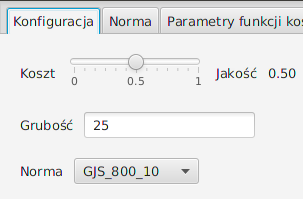
\includegraphics[scale=0.6]{images/conf.png}
        \caption {
            Konfiguracja
        }
        \label{fig:conf}
    \end{subfigure}
   \hfill
    \begin{subfigure}[b]{0.7\textwidth}
    	\centering
    	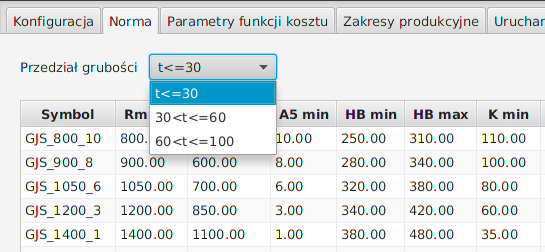
\includegraphics[scale=0.6]{images/norm.png}
    	\caption {
    		 Norma
    	}
    	\label{fig:norm}
    \end{subfigure}
    \vfill
    \begin{subfigure}[b]{0.3\textwidth}
    	\centering
    	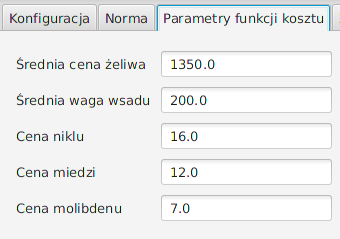
\includegraphics[scale=0.6]{images/cost.png}
    	\caption {
    		 Parametry funkcji kosztu
    	}
	    \label{fig:cost-tab}
    \end{subfigure}
    \hfill
    \begin{subfigure}[b]{0.7\textwidth}
    	\centering
    	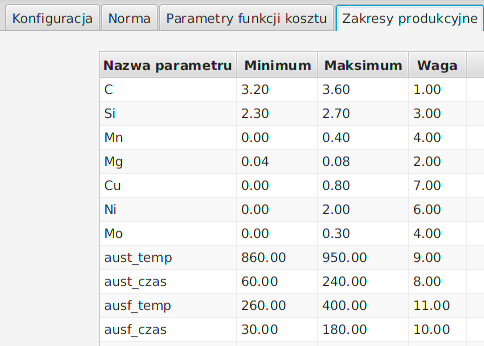
\includegraphics[scale=0.6]{images/prod_range.png}
    	\caption {
    		 Zakresy produkcyjne
    	}
    	\label{fig:prod-range-tab}
    \end{subfigure}
    \vfill
    \begin{subfigure}[b]{\textwidth}
    	\centering
    	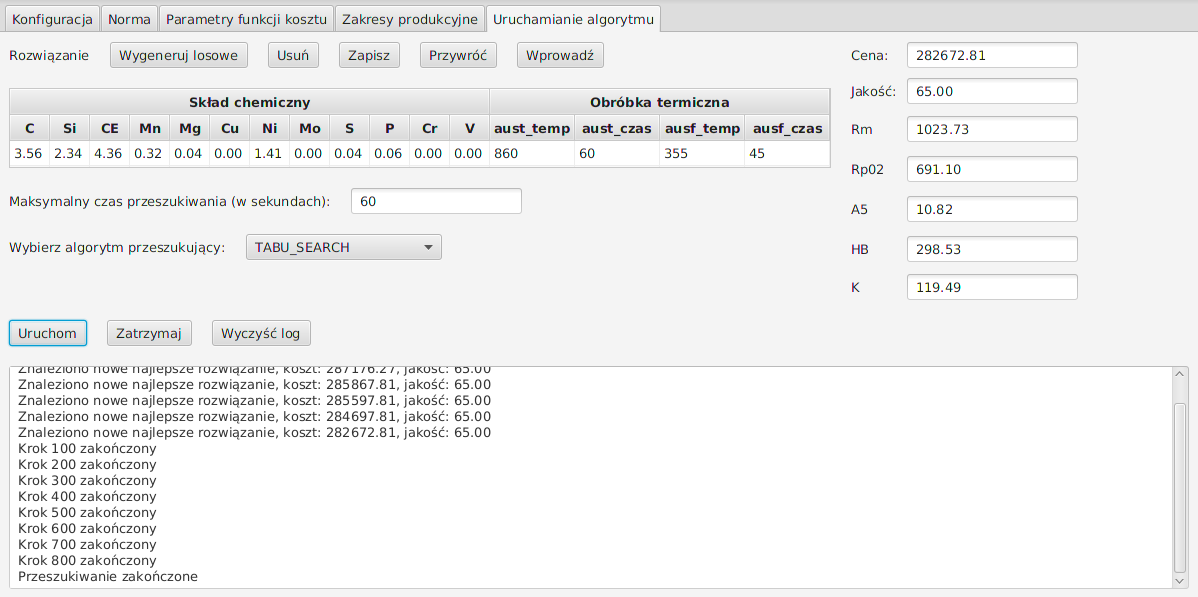
\includegraphics[scale=0.45]{images/algo_run.png}
    	\caption {
    		 Uruchamianie algorytmu
    	}
    	\label{fig:algo-run-tab}
    \end{subfigure}
    \caption{Zrzuty ekranu z graficznego interfejsu użytkownika}
    \label{fig:three graphs}
\end{figure}

Sposób uruchomienia i dodatkowe opisy zostały zawarte w załączniku na końcu pracy.

\FloatBarrier

\subsection{Ładowanie i używanie modeli w systemie}
Proces ładowania modeli odbywa się podczas ładowania systemu. Cała konfiguracja do tego służąca została zdefiniowana w postaci pliku o formacie JSON, w którym znajdują się ścieżki do modeli i ich konfiguracje warst wejściowych wraz z wartościami minimalnymi i maksymalnymi oraz przesunięciem, które służą do normalizacji wartości wejściowych modeli. Dodatkowo, w pliku konfiguracji znajduje się ścieżka do pliku w formacie JSON zawierającego wszystkie możliwe wartości, z których budowana jest przestrzeń rozwiązań dla algorytmów przeszukiwania. 

System obsługuje dwa źródła modeli:
\begin{itemize}
    \item modele wytrenowane za pomocą biblioteki XGBoost
    \item modele wytrenowane za pomocą biblioteki Keras
\end{itemize}

W pliku konfiguracyjnym należy podać typ modelu, czyli bibliotekę w której został wytrenowany. Przykładowa definicja modelu twardości została przedstawiona na rys. \ref{fig:hb-xgb}.

\begin{figure}[ht]{}
	\centering
	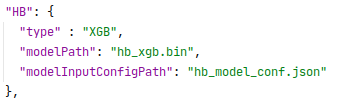
\includegraphics[scale=0.8]{images/hb-xgb.png}
	\caption {
		 Fragment konfiguracji systemu przedstawiający przykładową konfigurację modelu twardości.
	}
	\label{fig:hb-xgb}
\end{figure}






